\newcommand\el[2]{\text{#1}_{#2}}
\newcommand\sucrose{\overbrace{\el{C}{12}\el{H}{22}\el{O}{11}}^{\text{sucrose}}}
\newcommand\oxygen{\el{O}{2}}
\newcommand\carbonDioxide{\el{C}{}\el{O}{2}}
\newcommand\water{\el{H}{2}\el{O}{}}

\section{Chemistry}
Source: \href{https://www.youtube.com/watch?v=uVFCOfSuPTo&list=PL8dPuuaLjXtPHzzYuWy6fYEaX9mQQ8oGr}{Crash Course Chemistry}
\\\\
Chemistry is the scientific study of the \textbf{properties and behavior} of matter.

\subsection{The Periodic Table}
Source: \href{https://www.youtube.com/watch?v=0RRVV4Diomg&list=PL8dPuuaLjXtPHzzYuWy6fYEaX9mQQ8oGr&index=5}{The Periodic Table: Crash Course Chemistry \#4}\\
Source: \href{https://www.youtube.com/watch?v=rz4Dd1I_fX0}{The Periodic Table Song}
\\\\
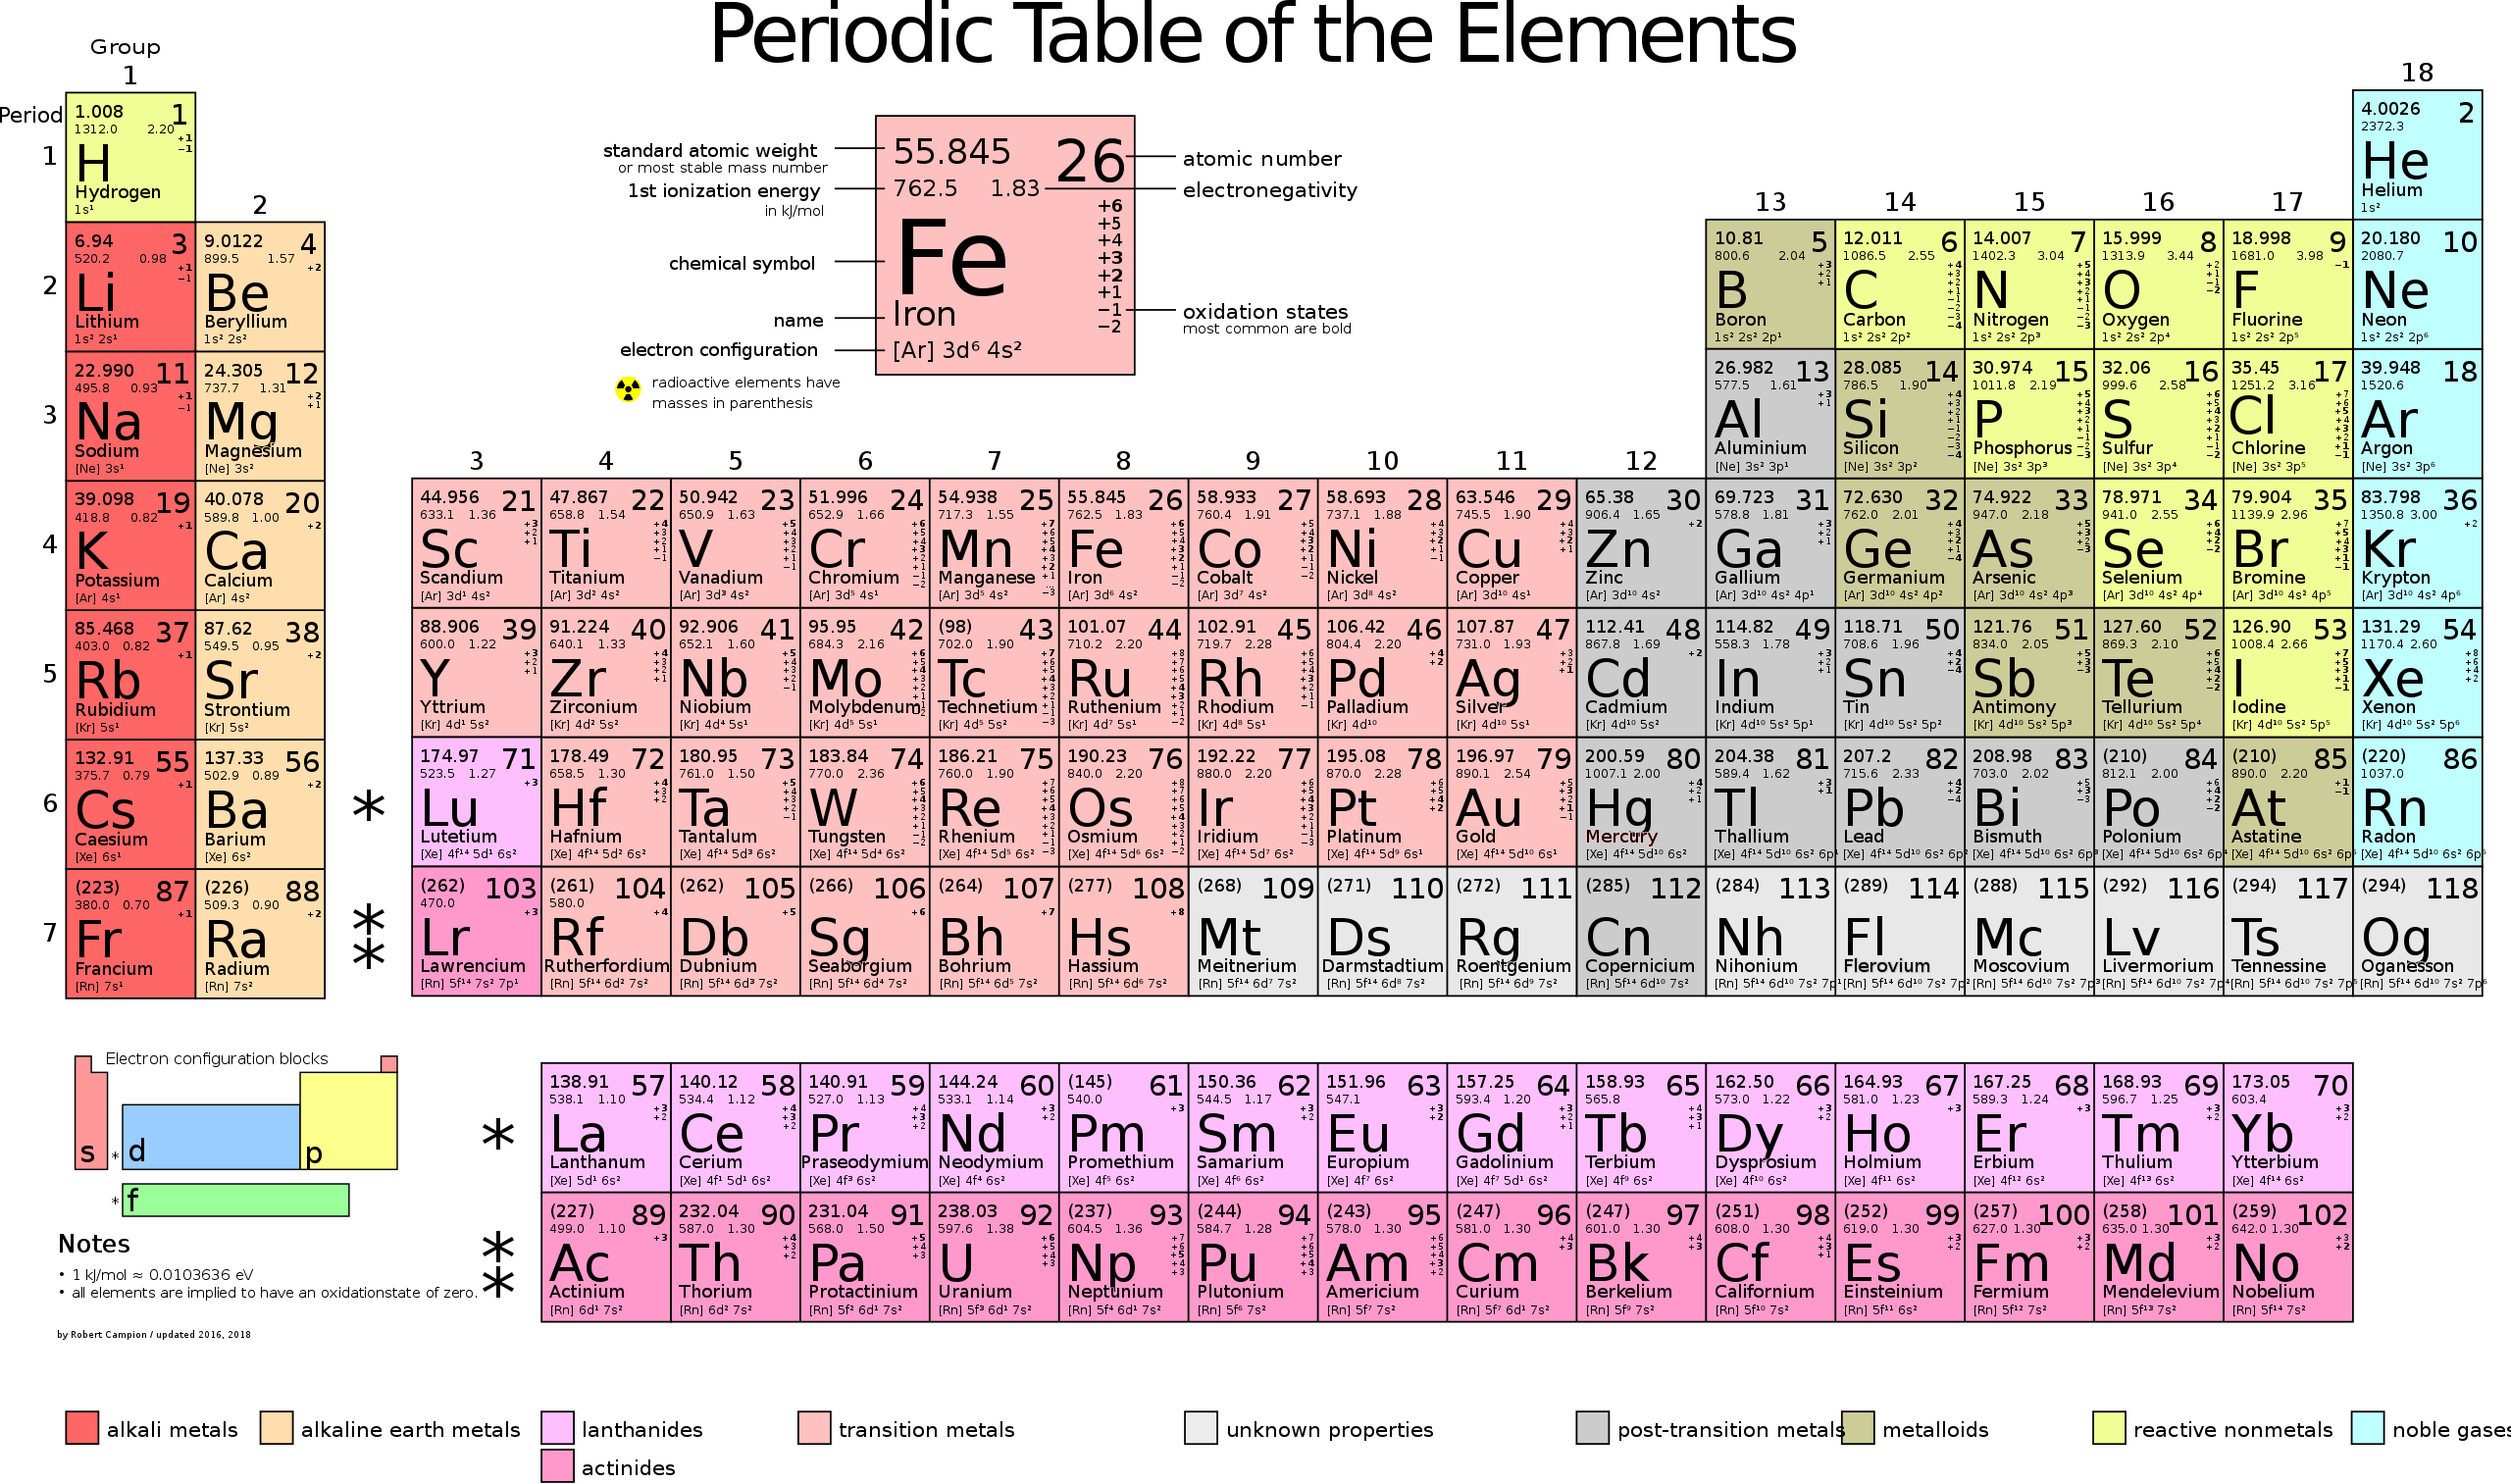
\includegraphics[width=\textwidth]{./chemistry/imgs/ptoe.png}
\\
Relative atomic mass (deprecated atomic weight) is ration to the atomic mass unit (amu), see Stoichiometry\\
Going down the table increases the radii of the atom (more shells).\\
Going right decreases the radii because more protons = more force inward.

\begin{description}
    \item[Dmitri Mendeleev] The Father of the Periodic Table.
    \item[Protons] atom type/number
    \item[neutron] stable / instable (isotopes)
    \item[electron] negative (cation + \& anion-, ions)
    \item[Alkali Metals] Also known as group IA
    \begin{description} 
        \item[] Very reactive, malleable, ductile, conductors
        \item[] Can explode when exposed to water (especially Cesium and Francium)
        \item[] Stored in inert gas or oil
    \end{description}
    \item[Alkaline Earth Metals] Also known as group IIA
    \begin{description} 
        \item[] Smaller atomic radii than alkali metals
        \item[] Readily form divalent cations
    \end{description} 
    \item[Transition Metals] Side group
    \begin{description} 
        \item[] Fairly unreactive, malleable
        \item[] High melting point, conductive
        \item[] Wide oxidation range
        \item[] Low ionization energy
    \end{description}
    \item[Halogens] Also known as group VIIA
    \begin{description}
        \item[] Highly reactive with alkali and alkaline earth metals
    \end{description}
    \item[Nobel gas] Also known as group VIIIA
    \begin{description}
        \item[] Non-reactive
        \item[] High ionization energy
    \end{description}
\end{description}
%
Ionization energy increases up and right\\ 
Electron affinity increases up and right (except noble gas)(how easy to gain an extra electron)

\subsection{The Electron}
Source: \href{https://www.youtube.com/watch?v=rcKilE9CdaA&list=PL8dPuuaLjXtPHzzYuWy6fYEaX9mQQ8oGr&index=6}{The Electron: Crash Course Chemistry \#5}
\\\\
Each orbital describes where the electron is most likely to be found.
\\
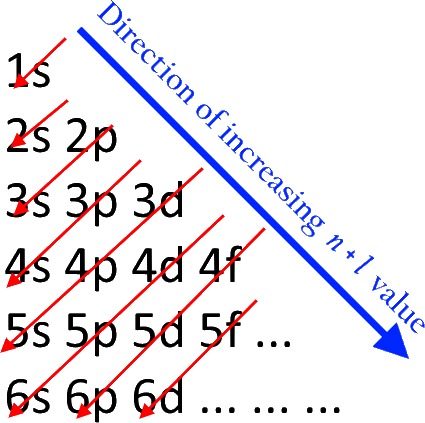
\includegraphics[width=10em]{./includes/chemistry/imgs/Aufbau_Principle.png}

\begin{description}
    \item[Aufbau Principle] Electrons fill orbitals of the lowest energy first.
    \item[Pauli Exclusion Principle] A maximum of two electrons with opposite spin can fit in an orbital.
    \item[Hund's Rule] Electrons will fill all orbitals of a sublevel with one electron before pairing up.
    \item[Octet rule] All tend to have 8 electrons in the outermost shell to become stable.
\end{description}
%
Number of electrons per shell: $2n^2$\\ 
The electron configuration $1\text{s}^2$ means: fist shell, s orbital, 2 electrons\\
The filling sequence is: $1\text{s}^1 \Rightarrow 1\text{s}^2 \Rightarrow 
1\text{s}^2 2\text{s}^1 \Rightarrow 1\text{s}^2 2\text{s}^ 2\Rightarrow 
1\text{s}^2 2\text{s}^2 2\text{p}^1$\\
But: $[\text{Ne}] 3\text{s}^2 3\text{p}^2 \Rightarrow [\text{Ar}] 4\text{s}^1 
\Rightarrow [\text{Ar}] 4\text{s}^2 \Rightarrow [\text{Ar}] 4\text{s}^2 3\text{d}^1$

\subsection{Stoichiometry}
Source: \href{https://www.youtube.com/watch?v=UL1jmJaUkaQ&list=PL8dPuuaLjXtPHzzYuWy6fYEaX9mQQ8oGr&index=7}{Stoichiometry - Chemistry for Massive Creatures: Crash Course Chemistry \#6}
\\\\
Stoichiometry is the relationship between the quantities of reactants and products before, during, and following chemical reactions.

\begin{description}
    \item[amu] $1.66 \cdot 10^{-27}kg =$ 1/12 the mass of an atom of $^{12}C$
    \item[mol] $6.022 \cdot 10^{23}$ (Avogadro's number)
    \item[Relative atomic mass] ram (deprecated atomic weight) is the ratio to the atomic mass unit (amu)
    \item[Molar mass] $\text{mol} \cdot \text{Relative atomic mass} =$ (Weight of one mol of the element)
    \item[Molarity] $M = \dfrac{\text{solute in moles}}{\text{solution\space in\space liters}}$
    \item[Molality]  $m = \dfrac{\text{solute in moles}}{\text{kg of solution}}$
    \item[Equation balancing] atom on lhs = atoms on rhs\\
        %$C_{12}H_{22}O_{11} + 12 O_{2} = 12 CO_{2} + 11 H_{2}O$\\
        $\sucrose + 12\oxygen = 12\carbonDioxide + 11\water$\\
        It means that to burn 5g of sucrose you need 5.6g of oxygen $\approx$ 35 breaths
\end{description}
%
Weight of one mol of $\sucrose = \text{C} + \text{H} + \text{O}$\\
$\text{C} = 12 \text{mol} \cdot 12.01\text{g/mol} = 144.12\text{g}$\\
$\text{H} = 22 \text{mol} \cdot 1.008\text{g/mol} = 22.176\text{g}$\\
$\text{O} = 11 \text{mol} \cdot 16.00\text{g/mol} = 171\text{g}$\\
One mol of sucrose = 342.296g

\subsubsection{Exothermic \& Endothermic}
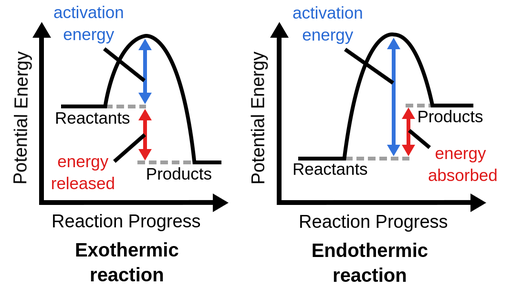
\includegraphics[width=30em]{./includes/chemistry/imgs/exo_endo.png}

\subsection{Mixtures}
Source: \href{https://en.wikipedia.org/wiki/Mixture#Homogeneous_and_heterogeneous_mixtures}{Wiki Mixture}
\\
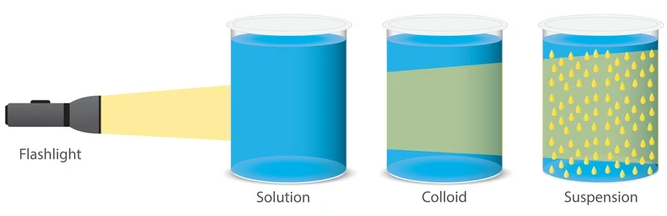
\includegraphics[width=40em]{./includes/chemistry/imgs/colloid.png}\\
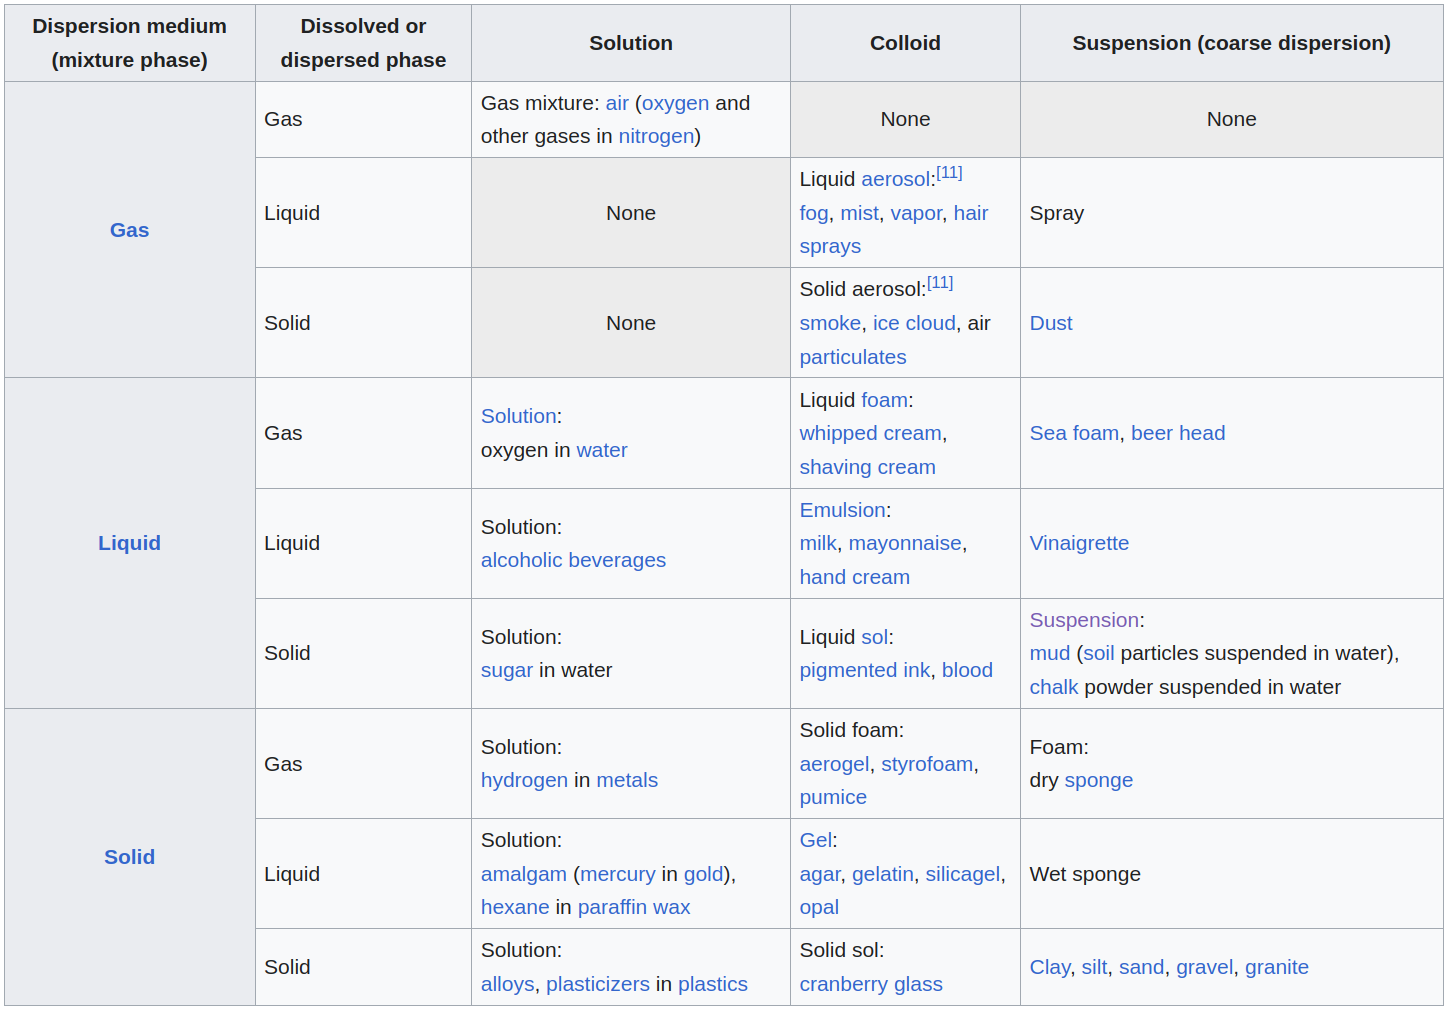
\includegraphics[width=\textwidth]{./includes/chemistry/imgs/mixtures.png}

\subsubsection{Separation methods}
Source: \href{https://byjus.com/chemistry/methods-of-separation/}{Separation methods}

\begin{description}
    \item[Handpicking] 
    \item[Threshing] Beating stalk to shake the grain off
    \item[Winnowing] Cleared from husk by falling through wind (husk fly away)
    \item[Sieving]
    \item[Evaporation / Fractionation] Different boiling point 
    \item[Distillation]
    \item[Sedimentation]
    \item[Separating Funnel] In a funnel different liquids separate and can be drained separately 
    \item[Magnetic Separation]
\end{description}

% TODO: Fix this subsection
\subsection{Bonds}
Source: \href{https://en.wikipedia.org/wiki/Chemical_bond}{Wiki: Chemical bond}

\subsubsection{Covalent bonding}
These type of bonds are made between non-metal elements.\\
Vdw Force is present

\begin{description}
    \item[non-polar] small electronegativity difference ($<$ 0.3)
    \item[polar] greater electronegativity difference, have dipole-dipole interaction\\
        Like $\text{H}_2\text{O}$\\
        Just means asymmetrical charge, but the total = 0
\end{description}

\subsubsection{Ionic bonding}
These type of bonds are made between non-metal and metal elements.
\\
Vdw Force is present\\
if H atoms on N/O/F/[Cl] the Hydrogen bond [H-Brücke] forces are present\\ 
The naming convention is cations than anions.\\

\begin{description}
    \item[] Salts
    \item[] Ions (Cations+,Anions-)
    \item[] Dissolved in water, they conduct electricity
    \item[] They are brittle [Spröd]
    \item[] NaCl \arrow sodium chloride
\end{description}
%
If we have N/S/P followed by O are nitrate/sulfate/phosphate which are anions.\\
Nitrate dissolve really easily in water.

\subsubsection{Metal bonding}
This bond is made between metal elements.

\begin{description}
    \item[] Atomic cores [Atomrümpfe]
    \item[] Electron gas \arrow give away valence electrons easily
    \item[] Generally electrically and heat conductive
\end{description}

\subsubsection{Geometry}
The shape of the molecule is determined by the central atom.
\\
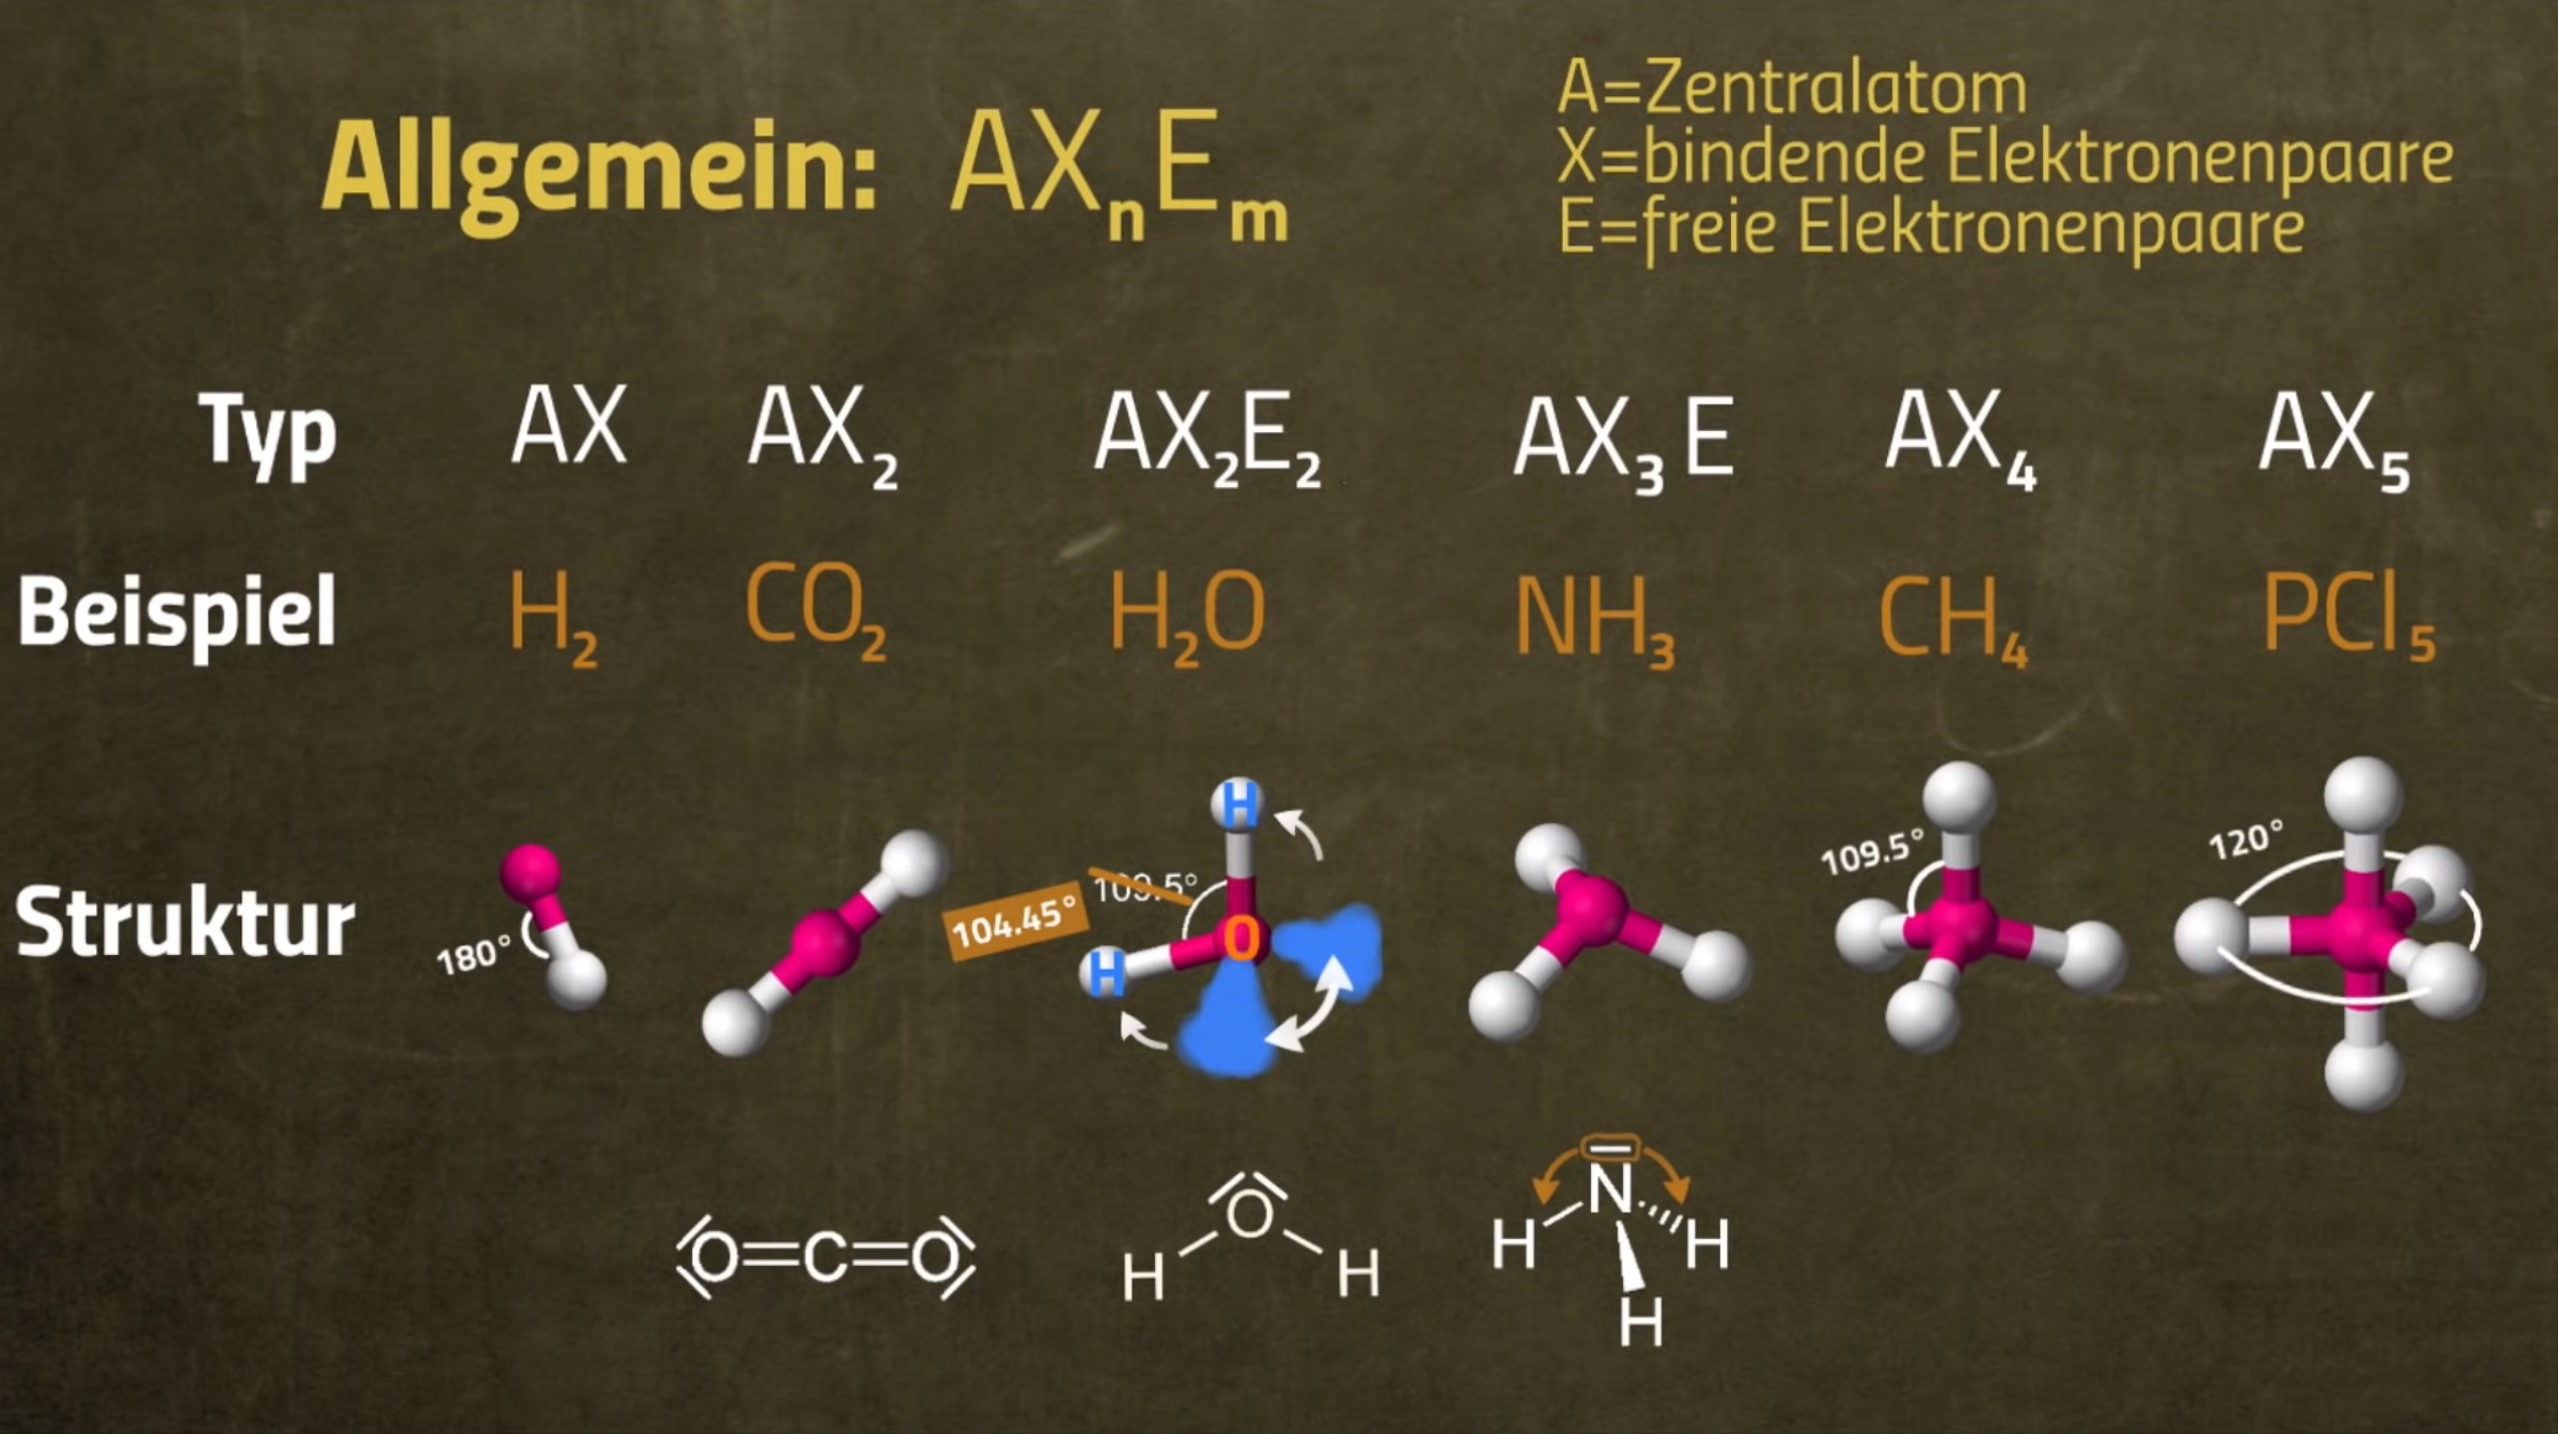
\includegraphics[width=30em]{./includes/chemistry/imgs/geometry.png}

\subsection{Reactions}

\subsubsection{Solution}
Source: \href{https://www.youtube.com/watch?v=AN4KifV12DA&list=PL8dPuuaLjXtPHzzYuWy6fYEaX9mQQ8oGr&index=8}{Water \& Solutions - for Dirty Laundry: Crash Course Chemistry \#7}

\begin{description}
    \item[] solute in solvent = solution 
    \item[] water is polar \arrow great solvent \arrow aqueous solution
    \item[] similar dissolve
    \begin{description}
        \item[polar] water \arrow hydrophilic, lipophobic
        \item[non-polar] fat \arrow lipophilic, hydrophobic
    \end{description}
    \item[] ions in solution are electrolytes \arrow salts make water conductive \arrow dielectric property
    \item[] hydration energy $>$ lattice energy \arrow enthalpy is negative \arrow heat is released
    \item[] hydration energy $<$ lattice energy \arrow enthalpy is positive \arrow heat is absorbed
\end{description}

\subsubsection{Acid-Base}
Source: \href{https://www.youtube.com/watch?v=ANi709MYnWg&list=PL8dPuuaLjXtPHzzYuWy6fYEaX9mQQ8oGr&index=9}{Acid-Base Reactions in Solution: Crash Course Chemistry \#8}

\begin{description}
    \item[acid] anything that donates a Proton
    \item[base] anything that accepts a Proton 
    \item[$\text{H}^+$] Protons in solution \arrow Hydrogen atom without electron \arrow Hydronium \arrow Proton
    \item[Conjugate acid] $\text{H}_3\text{O}^+ \qquad \text{N}\text{H}_4^+$ 
    \item[Conjugate base] $\text{C}\text{L}^- \qquad \text{O}\text{H}^-$ 
\end{description}

\subsubsection{Precipitation}
Source: \href{https://www.youtube.com/watch?v=IIu16dy3ThI&list=PL8dPuuaLjXtPHzzYuWy6fYEaX9mQQ8oGr&index=10}{Precipitation Reactions: Crash Course Chemistry \#9}
\\
Stuff falling out of other stuff as solid precipitate!\\
$\text{AgNO}_{3(aq)}+\text{NaCl}_{(aq)} \to \text{NaNo}_{3(aq)} + \text{AgCl}_{(s)}$
\subsubsection{Redox}
Source: \href{https://www.youtube.com/watch?v=lQ6FBA1HM3s&list=PL8dPuuaLjXtPHzzYuWy6fYEaX9mQQ8oGr&index=11}{Redox Reactions: Crash Course Chemistry \#10}
\\
OIL RIG = Oxidation Is Loss of electrons, Redux Is Gain of electrons

\subsubsection{Electrical current in salty solutions}

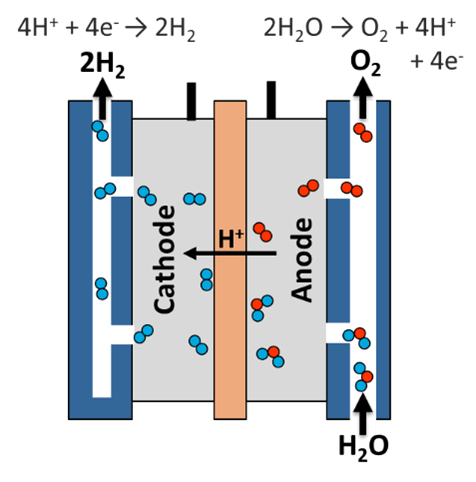
\includegraphics{./includes/chemistry/imgs/electrolyzer.png}
\\
Here the electrons flow from the Cathode- to the Anode+ (Through the wire).\\
The protons H+ flow from the Anode to the Cathode (through the electrolyte).

\subsection{Random}
- Water is at its densest at 4°C and ice floats on water

\begin{description}
    \item[Brownian motion] random motion of particles suspended in a medium
\end{description}